% Options for packages loaded elsewhere
\PassOptionsToPackage{unicode}{hyperref}
\PassOptionsToPackage{hyphens}{url}
%
\documentclass[
]{article}
\usepackage{lmodern}
\usepackage{amssymb,amsmath}
\usepackage{ifxetex,ifluatex}
\ifnum 0\ifxetex 1\fi\ifluatex 1\fi=0 % if pdftex
  \usepackage[T1]{fontenc}
  \usepackage[utf8]{inputenc}
  \usepackage{textcomp} % provide euro and other symbols
\else % if luatex or xetex
  \usepackage{unicode-math}
  \defaultfontfeatures{Scale=MatchLowercase}
  \defaultfontfeatures[\rmfamily]{Ligatures=TeX,Scale=1}
\fi
% Use upquote if available, for straight quotes in verbatim environments
\IfFileExists{upquote.sty}{\usepackage{upquote}}{}
\IfFileExists{microtype.sty}{% use microtype if available
  \usepackage[]{microtype}
  \UseMicrotypeSet[protrusion]{basicmath} % disable protrusion for tt fonts
}{}
\makeatletter
\@ifundefined{KOMAClassName}{% if non-KOMA class
  \IfFileExists{parskip.sty}{%
    \usepackage{parskip}
  }{% else
    \setlength{\parindent}{0pt}
    \setlength{\parskip}{6pt plus 2pt minus 1pt}}
}{% if KOMA class
  \KOMAoptions{parskip=half}}
\makeatother
\usepackage{xcolor}
\IfFileExists{xurl.sty}{\usepackage{xurl}}{} % add URL line breaks if available
\IfFileExists{bookmark.sty}{\usepackage{bookmark}}{\usepackage{hyperref}}
\hypersetup{
  pdftitle={Estatística e Análise de Dados},
  pdfauthor={Lirielly Nascimento e Pedro Magalhães},
  hidelinks,
  pdfcreator={LaTeX via pandoc}}
\urlstyle{same} % disable monospaced font for URLs
\usepackage[margin=2.5cm]{geometry}
\usepackage{longtable,booktabs}
% Correct order of tables after \paragraph or \subparagraph
\usepackage{etoolbox}
\makeatletter
\patchcmd\longtable{\par}{\if@noskipsec\mbox{}\fi\par}{}{}
\makeatother
% Allow footnotes in longtable head/foot
\IfFileExists{footnotehyper.sty}{\usepackage{footnotehyper}}{\usepackage{footnote}}
\makesavenoteenv{longtable}
\setlength{\emergencystretch}{3em} % prevent overfull lines
\providecommand{\tightlist}{%
  \setlength{\itemsep}{0pt}\setlength{\parskip}{0pt}}
\setcounter{secnumdepth}{5}
%----------------------------------------------------------------------------------------
%	REQUIRED PACKAGES
%
% pdfpages:(http://mirrors.up.pt/pub/CTAN/macros/latex/contrib/pdfpages/pdfpages.pdf)
% geometry: (https://www.overleaf.com/learn/latex/Page_size_and_margins)
% fancyhdr: (https://www.overleaf.com/learn/latex/Headers_and_footers)
% xcolor: (https://www.overleaf.com/learn/latex/Using_colours_in_LaTeX)
% titlesec: https://www.overleaf.com/learn/latex/Sections_and_chapters
%----------------------------------------------------------------------------------------

\usepackage{pdfpages} %allows the introduction of pdf pages 
\usepackage{fancyhdr} %changes headers and footers
\usepackage{xcolor} %Lets set different colors for the document
\usepackage{titlesec} %customizes chapters(book) and sections(article)
\usepackage{tikz}
\usepackage{fontspec} %customizes fonts
\usepackage{graphicx} %add graphical elements
\usepackage{background} %customizes documents backgrounds
\usepackage{lastpage}
\usepackage{caption} % allows image caption costumization
\usepackage{blindtext}
\usepackage[most]{tcolorbox}
\tcbuselibrary{skins}
\usepackage{multicol} % allows more than one column on text
\usepackage{enumitem} % Allows to change lists %>% 
\usepackage[default]{opensans}
\usepackage{setspace}\setstretch{1.25}
\usepackage{float}
\floatplacement{figure}{H}
%\usepackage{setspace}\singlespacing

%----------------------------------------------------------------------------------------
%	FONTS FORMAT
%----------------------------------------------------------------------------------------

\setmainfont[SizeFeatures={Size=10}]{Open Sans}

%----------------------------------------------------------------------------------------
%	DOCUMENT COLORS
%----------------------------------------------------------------------------------------

\definecolor{DarkPurple}{HTML}{680c62}
\definecolor{MediumPurple}{HTML}{a8139d}
\definecolor{LightPurple}{HTML}{c26cf0}
\definecolor{Grey}{HTML}{bfbfbf}
\definecolor{lightGreen}{HTML}{ddeedd}
\definecolor{mediumGreen}{HTML}{77bb77}

\definecolor{DarkGray}{HTML}{403D3C}
\definecolor{AtomicGreen}{HTML}{10FF10}

%----------------------------------------------------------------------------------------
%	SECTION FORMAT
%----------------------------------------------------------------------------------------

\titleformat{\section}[block]
  {\titlerule\addvspace{4pt}\normalfont\fontsize{12}{12}\bfseries}
  {\thesection\enspace}{0pt}{}[\vspace{2pt}\titlerule]

\titleformat*{\section}{\color{DarkGray}\fontsize{16}{16}\normalfont\bfseries}
\titleformat*{\subsection}{\color{DarkGray}\fontsize{12}{12}\normalfont\bfseries}
\titleformat*{\subsubsection}{\color{AtomicGreen}\fontsize{10}{10}\normalfont\bfseries}

\titlespacing*{\section}{0pt}{30pt}{50pt}
\titlespacing*{\subsection}{0pt}{40pt}{10pt}

%----------------------------------------------------------------------------------------
%	CUSTOM HEADER AND FOOTER
%----------------------------------------------------------------------------------------

\pagestyle{fancy}
\fancyhf{} %clear all headers and footer fields
%\fancyhead[RO,RE]{\textcolor{DarkGray}{math.marketing}}
\fancyhead[LO,LE]{\textcolor{DarkGray}{\thepage}}
\renewcommand{\headrulewidth}{0pt} %Eliminates header row that is part of the default


\backgroundsetup{
  scale=1.3,
  opacity=1,
  angle=0,
  position=current page.south,
  hshift=0pt, %-27
  vshift=20pt,
  contents={%
  \small\sffamily%
  \begin{minipage}{1\textwidth}
  \includegraphics[scale=0.5]{theme/images/footer.png}
  \end{minipage}%
  }
}

%----------------------------------------------------------------------------------------
%	CUSTOM IMAGE FORMATING
%----------------------------------------------------------------------------------------

\captionsetup[figure]{name=Fig.}

%----------------------------------------------------------------------------------------
%	COVER PAGE
%----------------------------------------------------------------------------------------

\AtBeginDocument{\let\maketitle\relax}

%----------------------------------------------------------------------------------------
%	NEW COMMANDS
%-------------------------------------------------------------------------------------

% http://texdoc.net/texmf-dist/doc/latex/tcolorbox/tcolorbox.pdf

\newcommand{\impactBox}[2]{
  \begin{tcolorbox}[width=\textwidth,
  fonttitle = \sffamily\bfseries\large, 
  colframe={mediumGreen},
  colback={lightGreen},
  title={#1},
  sharp corners]  
  \textsc{#2}
  \end{tcolorbox} 
}

\newcommand{\attentionBox}[1]{
  \begin{tcolorbox}[fonttitle = \sffamily\bfseries\large,
  bicolor,
  sidebyside,
  lefthand width=0.5cm,
  sharp corners,
  boxrule=.4pt,
  colback=yellow!30,
  colbacklower=yellow!20]
    \includegraphics[scale=5]{theme/images/attention-sign.png}
  \tcblower
    \textsc{#1}%
  \end{tcolorbox}
}
\usepackage[]{natbib}
\bibliographystyle{plainnat}

\title{Estatística e Análise de Dados}
\usepackage{etoolbox}
\makeatletter
\providecommand{\subtitle}[1]{% add subtitle to \maketitle
  \apptocmd{\@title}{\par {\large #1 \par}}{}{}
}
\makeatother
\subtitle{Trabalho Prático}
\author{Lirielly Nascimento e Pedro Magalhães}
\date{18/04/2022}

\begin{document}
\NoBgThispage %does not apply background

\includepdf{theme/images/cover.pdf}
\maketitle



{
\setcounter{tocdepth}{3}
\tableofcontents
}
\newpage

\hypertarget{introduuxe7uxe3o}{%
\section*{Introdução}\label{introduuxe7uxe3o}}
\addcontentsline{toc}{section}{Introdução}

\hypertarget{descriuxe7uxe3o-dos-dados}{%
\subsection*{Descrição dos Dados}\label{descriuxe7uxe3o-dos-dados}}
\addcontentsline{toc}{subsection}{Descrição dos Dados}

O Complexo Bushveld, a maior intrusão máfico-ultramáfica em camadas do mundo, é anfitrião de numerosas camadas de cromitita, lateralmente contínuas e quimicamente semelhantes. Com base em sua posição estratigráfica as camadas são subdivididas em um grupo inferior, médio e superior (LG, MG e UG). Dentro desses grupos as camadas são numeradas sucessivamente -- da base ao topo de cada grupo.

Tentativas de discriminar entre camadas únicas com base em sua composição falharam - principalmente devido à sobreposição significativa de campos de composição, por exemplo, de agrupamentos minerais de cromitita e química mineral de cromita entre camadas (vizinhas).

O conjunto de dados que utilizaremos foi fornecido pela Cronimet SA (Pty) Ltd., compreendendo em um grande banco de dados geoquímico (N = 1205) de cromitita de interseções de núcleo de perfuração e abrange 14 camadas de cromitita distintas (LG-1 -- LG-7, MG-1 -- MG-4, incluindo o LG-6A, MG-4A, MG-4Z) da Mina Thaba (que pode ser identificada na imagem abaixo), uma mina de cromita localizada no limbo ocidental do Complexo Bushveld. Os dados mostrados são restritos a cromitita maciça, excluindo paredões ou camadas suspensas de paredes, mas as análises podem conter intercalações de silicato finos (até alguns cm de espessura), separações de piroxenita, oikocristais de piroxênio, etc. Estes permanecem no conjunto de dados em ordem para representar toda a gama de possíveis composições de cromitita dentro da mina.

Durante a exploração na Mina Thaba, a composição das camadas de cromitita é rotineiramente restrita por apenas seis óxidos de elementos principais (Cr2O3, FeO, Al2O3, MgO, SiO2, CaO) e P. Além disso, o banco de dados da empresa contém valores para concentrações de Au e PGE, incluindo Pt, Pd, Rh, Ru e Ir. O banco de dados foi previamente filtrado para quaisquer valores ausentes (como ``não analisado'' ou ``abaixo do limite de detecção'') entre os principais óxidos do elemento e o PGE.

\begin{center}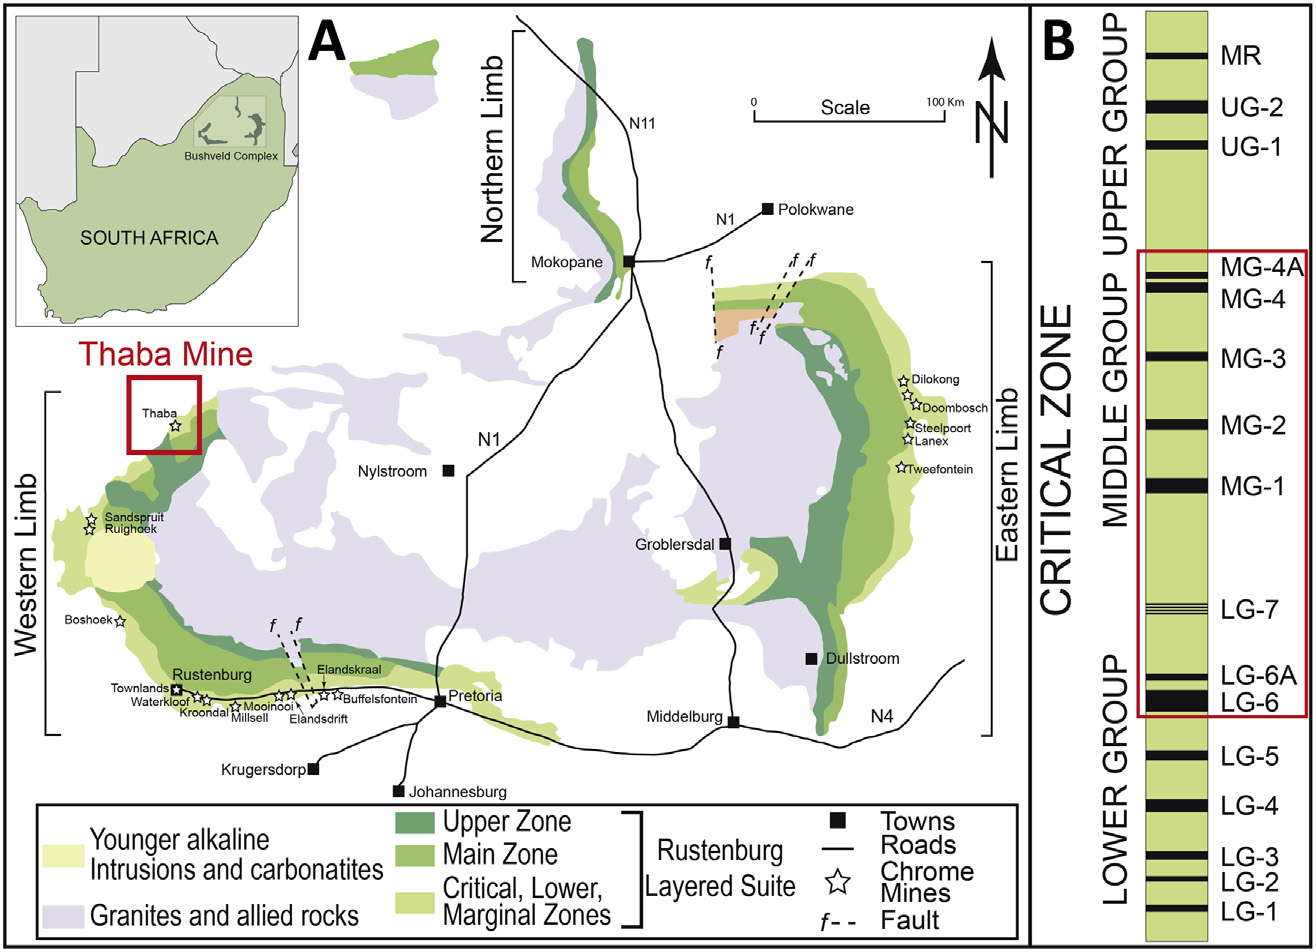
\includegraphics{./data/CB} \end{center}

Neste trabalho realizaremos algumas análises, dentre elas: análise de correlação, análise de componentes principais e análise do qui-quadrado. O nosso intuito com essas análises é verificar se conseguimos reduzir a dimensionalidade dos dados (variáveis numéricas) e obter um novo espaço de representação com uma boa representatividade das variáveis originais com as componentes criadas. Mais ainda, que as componentes selecionadas, as que explicam parte importante da dispersão, consigam mostrar a influência dos componentes geoquímicos nas amostras de cromitita.

O dataset contendo os dados analisados neste trabalho pode ser acessado no seguinte

\url{https://www.kaggle.com/saurabhshahane/multivariate-geochemical-classification}.

\hypertarget{definiuxe7uxe3o-das-variuxe1veis}{%
\subsection*{Definição das variáveis}\label{definiuxe7uxe3o-das-variuxe1veis}}
\addcontentsline{toc}{subsection}{Definição das variáveis}

\begin{itemize}
\item
  HoleType (Categórica): Tipo do furo que foi coletada a amostra
\item
  MaxDepth (Categórica): Profundidade máxima da coleta da amostra
\item
  DepthFrom (Numérica): Profundidade inicial da coleta da amostra
\item
  DepthTo (Numérica): Profundidade final da coleta da amostra
\item
  Cr2O3\_\% (Numérica): Percentual de Óxido de Cromo presente na amostra
\item
  FeO\_\% (Numérica): Percentual de Óxido de Ferro presente na amostra
\item
  SiO2\_\% (Numérica): Percentual de Dióxido de Silício presente na amostra
\item
  MgO\_\% (Numérica): Percentual de Óxido de Magnésio presente na amostra
\item
  Al2O3\_\% (Numérica: Percentual de Óxido de Alumínio presente na amostra
\item
  CaO\_\% (Numérica): Percentual de Óxido de Cálcio presente na amostra
\item
  P\_\% (Numérica): Percentual de Fósforo presente na amostra
\item
  Au\_ICP\_ppm (Numérica): Partes por milhão de ICP (Plasma Acoplado Indutivamente) de Ouro
\item
  Pt\_ICP\_ppm (Numérica): Partes por milhão de ICP (Plasma Acoplado Indutivamente) de Platina
\item
  Pd\_ICP\_ppm (Numérica): Partes por milhão de ICP (Plasma Acoplado Indutivamente) de Paládio
\item
  Rh\_ICP\_ppm (Numérica): Partes por milhão de ICP (Plasma Acoplado Indutivamente) de Ródio
\item
  Ir\_ICP\_ppm (Numérica): Partes por milhão de ICP (Plasma Acoplado Indutivamente) de Irídio
\item
  Ru\_ICP\_ppm (Numérica): Partes por milhão de ICP (Plasma Acoplado Indutivamente) de Ruténio
\item
  Stratigraphy (Categórica): Posição estratigráfica das camadas de cromitita dentro da Zona Crítica a partir da base para cima
\end{itemize}

\newpage

\hypertarget{data-exploration}{%
\section{Data Exploration}\label{data-exploration}}

\hypertarget{holetype}{%
\subsection{HoleType}\label{holetype}}

\begin{center}\includegraphics{_main_files/figure-latex/unnamed-chunk-5-1} \end{center}

A variável \textbf{Holetype} que representa o tipo do buraco feito para coleta da amostra de cromitita em uma das sessõe da mina do complexo de Bushveld. A variável é categórica sendo que a maior prediminância da classe sendo o buraco feito por meio de um \textbf{poço artesiano} e a outra classe sendo o buraco feito por meio de \textbf{deflexão}.

\hypertarget{maxdepth}{%
\subsection{MaxDepth}\label{maxdepth}}

\begin{center}\includegraphics{_main_files/figure-latex/unnamed-chunk-6-1} \end{center}

\textbf{MaxDepth} é a profundidade máxima do buraco utilizado para coleta da amostra de cromitita para a análise química. A váriável é categórica sendo que as classes \textbf{``Low''} e \textbf{``Middle''} tem praticamente a mesma proporção e a classe \textbf{``Depth''} tem aproximadamente o dobro da proporção das outras duas.

\hypertarget{depthfrom}{%
\subsection{DepthFrom}\label{depthfrom}}

\begin{center}\includegraphics{_main_files/figure-latex/unnamed-chunk-7-1} \end{center}

\textbf{DepthFrom} é a profundidade inicial de onde a amostra de cromitita foi coletada para a análise química. A váriável é contínua com distribuição gamma. O box-plot indica a presença de outliers, mas no contexto da coleta de amostras de cromitita para análise quimica esses valores não se confirmam como outliers e sim como prováveis de acontecer. Observamos por meio da distribuição desta variável que temos alguns valores com grande magnitude e desta forma a mediana e os valores máximo e mínimo são boas medidas de tendência central.

\hypertarget{depthto}{%
\subsection{DepthTo}\label{depthto}}

\begin{center}\includegraphics{_main_files/figure-latex/unnamed-chunk-8-1} \end{center}

\textbf{DepthTo} é a profundidade final de onde a amostra de cromitita foi coletada para a análise química. A váriável é contínua com distribuição gamma. O box-plot indica a presença de outliers, mas no contexto da coleta de amostras de cromitita para análise quimica esses valores não se confirmam como outliers e sim como prováveis de acontecer. Observamos por meio da distribuição desta variável que temos alguns valores com grande magnitude e desta forma a mediana e os valores máximo e mínimo são boas medidas de tendência central.

\hypertarget{cr2o3_}\label{cr2o3_}}

\begin{center}\includegraphics{_main_files/figure-latex/unnamed-chunk-9-1} \end{center}

\textbf{Cr2O3\_\%} representa o percentual de \textbf{óxido de cromo} contido na amostra de cromitita analisada. A váriável é contínua com distribuição bimodal, o box-plot sugere a presença de outliers. Por possuir alguns valores de grande amplitude a mediana e os valores máximo e mínimo são boas medidas de tendência central.

\hypertarget{feo_}\label{feo_}}

\begin{center}\includegraphics{_main_files/figure-latex/unnamed-chunk-10-1} \end{center}

\textbf{FeO\_\%} representa o percentual de \textbf{óxido de ferro} contido na amostra de cromitita analisada. A váriável é contínua com distribuição normal, o box-plot sugere a presença de outliers. Como a distribuição desta variável se assemelha a uma distribuição normal a média e o desvio padrão são boas medidas de tendência central.

\hypertarget{sio2_}\label{sio2_}}

\begin{center}\includegraphics{_main_files/figure-latex/unnamed-chunk-11-1} \end{center}

\textbf{SiO2\_\%} representa o percentual de \textbf{dióxido de silício} contido na amostra de cromitita analisada. A váriável é contínua com distribuição bimodal, o box-plot sugere a presença de outliers. E, por possuir alguns valores de grande amplitude a mediana e os valores máximo e mínimo são boas medidas de tendência central.

\hypertarget{mgo_}\label{mgo_}}

\begin{center}\includegraphics{_main_files/figure-latex/unnamed-chunk-12-1} \end{center}

\textbf{MgO\_\%} representa o percentual de \textbf{óxido de magnésio} contido na amostra de cromitita analisada. A váriável é contínua com distribuição normal, o box-plot sugere a presença de outliers. Como a distribuição desta variável se assemelha a uma distribuição normal a média e o desvio padrão são boas medidas de tendência central.

\hypertarget{al2o3_}\label{al2o3_}}

\begin{center}\includegraphics{_main_files/figure-latex/unnamed-chunk-13-1} \end{center}

\textbf{Al2O3\_\%} representa o percentual de \textbf{óxido de alumínio} contido na amostra de cromitita analisada. A váriável é contínua com distribuição bimodal, o box-plot sugere a presença de outliers. E, por possuir alguns valores de grande amplitude a mediana e os valores máximo e mínimo são boas medidas de tendência central.

\hypertarget{cao_}\label{cao_}}

\begin{center}\includegraphics{_main_files/figure-latex/unnamed-chunk-14-1} \end{center}

\textbf{CaO\_\%} representa o percentual de \textbf{óxido de cálcio} contido na amostra de cromitita analisada. A váriável é contínua com distribuição bimodal, o box-plot sugere a presença de outliers. E, por possuir alguns valores de grande amplitude a mediana e os valores máximo e mínimo são boas medidas de tendência central.

\hypertarget{p_}\label{p_}}

\begin{center}\includegraphics{_main_files/figure-latex/unnamed-chunk-15-1} \end{center}

\textbf{P\_\%} representa o percentual de \textbf{fósfoto} contido na amostra de cromitita analisada. A váriável é contínua com distribuição similar a uma gamma ou poisson, o box-plot sugere a presença de outliers. E, por possuir alguns valores de grande amplitude a mediana e os valores máximo e mínimo são boas medidas de tendência central.

\hypertarget{au_icp_ppm}{%
\subsection{Au\_ICP\_ppm}\label{au_icp_ppm}}

\begin{center}\includegraphics{_main_files/figure-latex/unnamed-chunk-16-1} \end{center}

\textbf{Au\_ICP\_ppm} representa as partes por milhão de ICP (Plasma Acoplado Indutivamente) de \textbf{ouro} contido na amostra de cromitita analisada. A váriável é contínua com distribuição similar a uma gamma ou poisson, o box-plot sugere a presença de outliers. E, por possuir alguns valores de grande amplitude a mediana e os valores máximo e mínimo são boas medidas de tendência central.

\hypertarget{pt_icp_ppm}{%
\subsection{Pt\_ICP\_ppm}\label{pt_icp_ppm}}

\begin{center}\includegraphics{_main_files/figure-latex/unnamed-chunk-17-1} \end{center}

\textbf{Pt\_ICP\_ppm} representa as partes por milhão de ICP (Plasma Acoplado Indutivamente) de \textbf{platina} contido na amostra de cromitita analisada. A váriável é contínua com distribuição bimodal, o box-plot sugere a presença de outliers. E, por possuir alguns valores de grande amplitude a mediana e os valores máximo e mínimo são boas medidas de tendência central.

\hypertarget{pd_icp_ppm}{%
\subsection{Pd\_ICP\_ppm}\label{pd_icp_ppm}}

\begin{center}\includegraphics{_main_files/figure-latex/unnamed-chunk-18-1} \end{center}

\textbf{Pd\_ICP\_ppm} representa as partes por milhão de ICP (Plasma Acoplado Indutivamente) de \textbf{paládio} contido na amostra de cromitita analisada. A váriável é contínua com distribuição gamma, o box-plot sugere a presença de outliers. E, por possuir alguns valores de grande amplitude a mediana e os valores máximo e mínimo são boas medidas de tendência central.

\hypertarget{rh_icp_ppm}{%
\subsection{Rh\_ICP\_ppm}\label{rh_icp_ppm}}

\begin{center}\includegraphics{_main_files/figure-latex/unnamed-chunk-19-1} \end{center}

\textbf{Rh\_ICP\_ppm} representa as partes por milhão de ICP (Plasma Acoplado Indutivamente) de \textbf{ródio} contido na amostra de cromitita analisada. A váriável é contínua com distribuição gamma, o box-plot sugere a presença de outliers. E, por possuir alguns valores de grande amplitude a mediana e os valores máximo e mínimo são boas medidas de tendência central.

\hypertarget{ir_icp_ppm}{%
\subsection{Ir\_ICP\_ppm}\label{ir_icp_ppm}}

\begin{center}\includegraphics{_main_files/figure-latex/unnamed-chunk-20-1} \end{center}

\textbf{Ir\_ICP\_ppm} representa as partes por milhão de ICP (Plasma Acoplado Indutivamente) de \textbf{irídio} contido na amostra de cromitita analisada. A váriável é contínua com distribuição bimodal, o box-plot sugere a presença de outliers. E, por possuir alguns valores de grande amplitude a mediana e os valores máximo e mínimo são boas medidas de tendência central.

\hypertarget{ru_icp_ppm}{%
\subsection{Ru\_ICP\_ppm}\label{ru_icp_ppm}}

\begin{center}\includegraphics{_main_files/figure-latex/unnamed-chunk-21-1} \end{center}

\textbf{Ru\_ICP\_ppm} representa as partes por milhão de ICP (Plasma Acoplado Indutivamente) de \textbf{ruténio} contido na amostra de cromitita analisada. A váriável é contínua com distribuição gamma, o box-plot sugere a presença de outliers. E, por possuir alguns valores de grande amplitude a mediana e os valores máximo e mínimo são boas medidas de tendência central.

\textbf{Observação:} para todas as variáveis que representam as análises químicas tanto o percentual quanto as partes por milhão de ICP (Plasma Acoplado Indutivamente) vimos que o box-plot sugere a presença de outliers, porem esses valores atípicos podem desafiar um esquema de discriminação, mas parecem ser bastante comuns no Complexo Bushveld e são comumente atribuídos a heterogeneidades locais nos cromititos, por exemplo, a presença de grandes oikocristais de piroxênio ou uma concentração elevada de plagioclásio. E, por se tratar de fenômenos que podem ocorrer, nós não iremos eliminar os outlies dessas variáveis.

\hypertarget{stratigraphy}{%
\subsection{Stratigraphy}\label{stratigraphy}}

\begin{center}\includegraphics{_main_files/figure-latex/unnamed-chunk-22-1} \end{center}

\textbf{Stratigraphy} representa a posição estratigráfica das camadas de cromitita dentro da \textbf{Zona Crítica} a partir da base para cima. A váriável é categorica multiclasse. Através do gráfico de frequência observamos que existem 6 zonas críticas pouco frequentes, 4 zonas críticas com frequência média e 4 zonas críticas de alta frequência.

\hypertarget{martriz-de-correlauxe7uxe3o}{%
\subsection{Martriz de Correlação}\label{martriz-de-correlauxe7uxe3o}}

\begin{center}\includegraphics{_main_files/figure-latex/unnamed-chunk-23-1} \end{center}

\newpage

\hypertarget{anuxe1lise-componentes-principais}{%
\section{Análise Componentes Principais}\label{anuxe1lise-componentes-principais}}

\begin{verbatim}
##         p.value Variavel.1   Variavel.2
## 1  3.917371e-02 Motherhole     HoleType
## 2 1.425427e-211 Motherhole     MaxDepth
## 3  3.330420e-74 Motherhole Stratigraphy
## 4  1.941203e-08   HoleType     MaxDepth
## 5  7.670179e-81   HoleType Stratigraphy
## 6  1.511055e-16   MaxDepth Stratigraphy
\end{verbatim}

Analisando os testes qui-quadrados de todas as combinações das variáveis rejeitamos todas as hipóteses nulas correspondentes aos pares de variáveis analisadas nos testes qui-quadrados, pois \textbf{p-value \textless{} 0.05}. A hipótese Ho rejeitada afirma que o par te variáveis analisada no teste são idependentes.

\begin{verbatim}
## Warning in PCA(data %>% select_if(is.numeric), ncp = 7): Missing values are imputed by the mean of the
## variable: you should use the imputePCA function of the missMDA package
\end{verbatim}

\begin{center}\includegraphics{_main_files/figure-latex/unnamed-chunk-27-1} \includegraphics{_main_files/figure-latex/unnamed-chunk-27-2} \end{center}

As correlações geralmente são representadas em gráficos de círculo de correlações. No gráfico acima, temos o círculo de correlação entre a componente 1 e 2. O interessante nesse gráfico é analisar as correlações que se opõe via sinal. Dessa forma, podemos ver pela primeira componente que todos os ppm (ouro, platina, paládio, ródio, irídio e ruténio) e o óxido de alumínio são opostos ao fósforo e óxido de magnésio, ou seja, notamos que amostras tem maior concentração distintas desses elementos, os primeiros mencionados em maior concentração e os últimos em menor concentração.

Já a componente 2 nos mostra uma oposição entre profundidade, óxido de cromo e óxido de ferro em oposição a óxido de cálcio e óxido de silício seguindo a mesma ideia da explicação anterior.

\hypertarget{eigenvectors}{%
\subsection{Eigenvectors}\label{eigenvectors}}

\begin{verbatim}
##              [,1]        [,2]        [,3]        [,4]         [,5]        [,6]        [,7]
##  [1,] -0.33933464  0.12144243  0.40328377 -0.05249124  0.314385895  0.25349861 -0.13422250
##  [2,] -0.33960722  0.12146945  0.40289443 -0.05244141  0.314468732  0.25339654 -0.13397128
##  [3,] -0.35980699  0.32038227 -0.06073350 -0.02656228 -0.100308766 -0.16618602  0.06839196
##  [4,] -0.12121407  0.30975849 -0.28055012  0.39287508 -0.176845324  0.02796015 -0.23826212
##  [5,]  0.28172387 -0.38879095  0.22007052 -0.11606447  0.114030037  0.09231566  0.05968242
##  [6,] -0.02809692 -0.23626868  0.47648182  0.01527495 -0.313467441 -0.13456261  0.22685102
##  [7,]  0.17481993  0.20195233 -0.14962274 -0.46296814  0.227552638  0.05334712  0.11471749
##  [8,]  0.29638271 -0.26145947 -0.13353136  0.06785702  0.207484975  0.17912289 -0.11768858
##  [9,] -0.01077801 -0.04354203 -0.08247047  0.47093443 -0.066780813  0.69090318  0.42252561
## [10,]  0.01409460  0.01825290  0.05864187  0.42030567  0.511292863 -0.48332921  0.46830480
## [11,]  0.33598625  0.19712703  0.11564014  0.08658805  0.002006378  0.10715440 -0.27103454
## [12,]  0.26764658  0.16240325  0.22043419  0.35239272  0.169739138 -0.17603990 -0.28278312
## [13,]  0.34066948  0.28509924  0.23086802  0.11871804 -0.012734987  0.03293437 -0.16956314
## [14,]  0.32718617  0.34679038  0.15474522 -0.13023336 -0.096132840  0.08528446  0.21829363
## [15,]  0.13006313  0.40928033  0.15573183 -0.14413806 -0.191406478  0.02798404  0.42603748
## [16,]  0.04408344  0.13876677 -0.32133340 -0.15762334  0.462714050  0.13784494  0.10668008
\end{verbatim}

Podemos ver a tabela acima os 7 primeiros autovetores correspondentes aos autovalores em ordem decrescente. Sabemos que os autovetores estão normalizados e isso significa que a soma dos quadrados de cada componente do vetor é igual a 1. E, sabemos que eles são ortogonais, pois o produto de quaisquer dois autovetores, isto é a soma das componentes dos vetores multiplicadas termo a termo é sempre igual a zero. E isso significa que as componentes não estão correlacionadas entre si.

Com os autovetores nós conseguimos escrever as equações das componentes principais como combinação linear dos autovetores e as variáveis originais normalizadas.

\hypertarget{eigenvalues}{%
\subsection{Eigenvalues}\label{eigenvalues}}

\begin{verbatim}
##           eigenvalue percentage of variance cumulative percentage of variance
## comp 1  3.872695e+00           2.420434e+01                          24.20434
## comp 2  2.963345e+00           1.852091e+01                          42.72525
## comp 3  1.864835e+00           1.165522e+01                          54.38047
## comp 4  1.229058e+00           7.681614e+00                          62.06208
## comp 5  1.103187e+00           6.894921e+00                          68.95700
## comp 6  1.036939e+00           6.480867e+00                          75.43787
## comp 7  8.088408e-01           5.055255e+00                          80.49312
## comp 8  7.611018e-01           4.756886e+00                          85.25001
## comp 9  6.420646e-01           4.012904e+00                          89.26291
## comp 10 6.052525e-01           3.782828e+00                          93.04574
## comp 11 4.208582e-01           2.630364e+00                          95.67610
## comp 12 2.918730e-01           1.824206e+00                          97.50031
## comp 13 2.083027e-01           1.301892e+00                          98.80220
## comp 14 1.141093e-01           7.131834e-01                          99.51538
## comp 15 7.753320e-02           4.845825e-01                          99.99997
## comp 16 5.237520e-06           3.273450e-05                         100.00000
\end{verbatim}

Analisando as medidas de correlação, pois estamos fazendo o PCA normatizado o que se justifica dado que algumas variáveis possuem unidades muito diferentes e dispersão muito diferente. Nós obtemos a lista dos 16 autovalores apresentados aqui de forma decrescente.

Ao analisarmos os autovalores, temos que se utilizarmos o critério de Kaiser, onde diz que devemos manter as componentes com autovalores acima de 1, \textbf{reteríamos apenas as 6 primeiras componentes principais}, pois dessa forma reteríamos as componentes mais informativas do que as variáveis originais, dado que estas possuem variância maior do que as originais.

Mas se considerarmos o critério de Pearson, onde diz devemos manter as componentes de forma que elas expliquem pelo menos 80\% da dispersão total, aí teríamos que \textbf{manter as 7 primeiras componentes principais} para atingir esse objetivo.

\begin{center}\includegraphics{_main_files/figure-latex/unnamed-chunk-30-1} \end{center}

Aqui temos um histograma onde podemos visualizar a amplitude de cada um dos auto valores e podemos ver que os 3 primeiros realmente se destacam dos demais já os seguintes vão diminuindo suas amplitudes gradativamente sem nenhuma alta discrepância de maneira a formar degraus como os 3 primeiros.

\hypertarget{correlauxe7uxe3o-entre-as-componentes-principais-e-as-variuxe1veis-originais}{%
\subsection{Correlação entre as componentes principais e as variáveis originais}\label{correlauxe7uxe3o-entre-as-componentes-principais-e-as-variuxe1veis-originais}}

\begin{verbatim}
##             Dim.1  Dim.2  Dim.3  Dim.4  Dim.5  Dim.6  Dim.7
## DepthFrom  -0.668  0.209  0.551 -0.058  0.330  0.258 -0.121
## DepthTo    -0.668  0.209  0.550 -0.058  0.330  0.258 -0.120
## Cr2O3_%    -0.708  0.552 -0.083 -0.029 -0.105 -0.169  0.062
## FeO_%      -0.239  0.533 -0.383  0.436 -0.186  0.028 -0.214
## SiO2_%      0.554 -0.669  0.301 -0.129  0.120  0.094  0.054
## MgO_%      -0.055 -0.407  0.651  0.017 -0.329 -0.137  0.204
## Al2O3_%     0.344  0.348 -0.204 -0.513  0.239  0.054  0.103
## CaO_%       0.583 -0.450 -0.182  0.075  0.218  0.182 -0.106
## P_%        -0.021 -0.075 -0.113  0.522 -0.070  0.704  0.380
## Au_ICP_ppm  0.028  0.031  0.080  0.466  0.537 -0.492  0.421
## Pt_ICP_ppm  0.661  0.339  0.158  0.096  0.002  0.109 -0.244
## Pd_ICP_ppm  0.527  0.280  0.301  0.391  0.178 -0.179 -0.254
## Rh_ICP_ppm  0.670  0.491  0.315  0.132 -0.013  0.034 -0.152
## Ir_ICP_ppm  0.644  0.597  0.211 -0.144 -0.101  0.087  0.196
## Ru_ICP_ppm  0.256  0.705  0.213 -0.160 -0.201  0.028  0.383
## Filter      0.087  0.239 -0.439 -0.175  0.486  0.140  0.096
\end{verbatim}

Analisando os resultados de correlação entre as componentes principais e as variáveis originais da nossa base de dados, podemos concluir que:

\begin{enumerate}
\def\labelenumi{\arabic{enumi}.}
\item
  A componente principal 1 (\emph{Dim 1}) tem correlação forte negativa com as variáveis \textbf{DepthFrom, DepthTo, Cr2O3\_\%} e correlação forte positiva com as variáveis \textbf{CaO\_\%, SiO2\_\%, Pt\_ICP\_ppm, Pd\_ICP\_ppm, Rh\_ICP\_ppm, Ir\_ICP\_ppm}. Esta componente representa amostras com maior concentração de óxido de cromo, óxido de silício, ppm de platina, ppm de paládio, ppm de ródio e ppm de irídio, mas também com uma menor concentração de óxido de cromo e ainda representam amostras que foram coletadas em profundidades baixas, mais próximas da superfície.
\item
  A componente principal 2 (\emph{Dim 2}) possui correlação forte negativa com as seguintes variável \textbf{SiO2\_\%} e correlação forte positiva com as variáveis \textbf{Cr2O3\_\%, FeO\_\%, Ir\_ICP\_ppm, Ru\_ICP\_ppm}. O que representa somente elementos químicos presentes na análise de uma amostra de cromitita, são melhores representadas pela Dim 2 quando olhamos para as correlações. Sendo assim essa componente representa amostras com maior concentração de óxido de cromo, óxido de ferro, ppm de ruténio e ppm de irídio, mas também com menor concentração de óxido de silício.
\item
  Para a componente principal 3 (\emph{Dim 3}) temos uma apenas correlação forte positiva com as variáveis \textbf{DepthFrom, DepthTo, MgO\_\%}. Sendo assim essa componente identifica amostras com maiores concentrações de óxido de magnésio e amostras retiradas de locais mais profundos, mais distantes da superfície.
\item
  Para a componente principal 4 (\emph{Dim 4}) vemos uma maior correlação positiva da variável P\_\% e uma correlação forte negativa da variável \textbf{Al2O3\_\%} então essa componente descreve amostras com maiores concentrações de fósforo e menores concentrações de óxido de alumínio.
\item
  Para a componente principal 5 (\emph{Dim 5}) podemos ver que temos uma maior correlação positiva com a variável \textbf{Au\_ICP\_ppm}, desta forma essa componente consegue identificar amostras com uma maior concentração de ppm de ouro.
\item
  Para a componente principal 6 (\emph{Dim 6}) temos uma correlação forte positiva com a variável \textbf{P\_\%}, sendo assim essa componente consegue representar amostras com maior concentração de fósforo.
\item
  E por fim a componente principal 7 (\emph{Dim 7}) não possui correlação forte nem positiva nem negativa com nenhuma das variáveis originais.
\end{enumerate}

\hypertarget{contribuiuxe7uxe3o-presente-nas-componentes-principais}{%
\subsection{Contribuição presente nas componentes principais}\label{contribuiuxe7uxe3o-presente-nas-componentes-principais}}

\begin{verbatim}
##             Dim.1  Dim.2  Dim.3  Dim.4  Dim.5  Dim.6  Dim.7
## DepthFrom  11.515  1.475 16.264  0.276  9.884  6.426  1.802
## DepthTo    11.533  1.475 16.232  0.275  9.889  6.421  1.795
## Cr2O3_%    12.946 10.264  0.369  0.071  1.006  2.762  0.468
## FeO_%       1.469  9.595  7.871 15.435  3.127  0.078  5.677
## SiO2_%      7.937 15.116  4.843  1.347  1.300  0.852  0.356
## MgO_%       0.079  5.582 22.703  0.023  9.826  1.811  5.146
## Al2O3_%     3.056  4.078  2.239 21.434  5.178  0.285  1.316
## CaO_%       8.784  6.836  1.783  0.460  4.305  3.209  1.385
## P_%         0.012  0.190  0.680 22.178  0.446 47.735 17.853
## Au_ICP_ppm  0.020  0.033  0.344 17.666 26.142 23.361 21.931
## Pt_ICP_ppm 11.289  3.886  1.337  0.750  0.000  1.148  7.346
## Pd_ICP_ppm  7.163  2.637  4.859 12.418  2.881  3.099  7.997
## Rh_ICP_ppm 11.606  8.128  5.330  1.409  0.016  0.108  2.875
## Ir_ICP_ppm 10.705 12.026  2.395  1.696  0.924  0.727  4.765
## Ru_ICP_ppm  1.692 16.751  2.425  2.078  3.664  0.078 18.151
## Filter      0.194  1.926 10.326  2.485 21.410  1.900  1.138
\end{verbatim}

Aqui podemos ver que na componente principal 1 (\emph{Dim 1}) as variáveis que representam a profundidade, óxido de cromo, ppm de platina, ppm de ródio e ppm de irídio correspondem as variáveis que tem contribuições mais importantes para a componente e ainda são as mesmas variáveis que possuem maiores correlação. Analogamente essa análise pode ser feita para as demais componentes, seguindo o mesmo raciocínio.

\hypertarget{gruxe1fico-pca-dos-indivuxedduos}{%
\subsection{Gráfico PCA dos indivíduos}\label{gruxe1fico-pca-dos-indivuxedduos}}

\begin{center}\includegraphics{_main_files/figure-latex/unnamed-chunk-33-1} \end{center}

No gráfico de indivíduos acima conseguimos observar que os indivíduos \textbf{1136 e 651} tem alta concentração dos ppm (ouro, platina, paládio, ródio, irídio e ruténio) e de óxido de alumínio isso porque a componente 1 nos mostra isso. E, os indivíduos \textbf{534, 745 e 160} tem menores concentrações de óxido de cálcio e óxido de silício. Os outros indivíduos como estão bastante concentrados nos quadrantes de 1 a 4 não conseguimos os identificar para uma análise apropriada.

\begin{center}\includegraphics{_main_files/figure-latex/unnamed-chunk-34-1} \end{center}

Aqui temos que o indivíduo \textbf{881} tem uma alta concetração de óxido de ferro e fósforo. Enquanto os indíviduos \textbf{657 e 1143} tem uma alta concentração de ppm de ouro, ppm de paládio e óxido de manganês.

\begin{center}\includegraphics{_main_files/figure-latex/unnamed-chunk-35-1} \end{center}

Já nesté gráfico dos indivíduos representados pelas componentes 5 e 6, podemos observar que o indivíduo \textbf{881} tem uma alta concentração de fósforo indicada pela componente 6, os indivíduos \textbf{275, 105 e 647} tem uma alta concentração de ppm de outro indicada pela componente 5.

\newpage

\end{document}
